% Generazione delle variabili che andranno a sostituire quelle del template `HomePage.tex`
\newcommand{\documento}{\MU}
\newcommand{\nomedocumentofisico}{\MUv.pdf}
\newcommand{\redazione}{\TG \\ & \CV}
\newcommand{\verifica}{\LC \\ & \NC}
\newcommand{\approvazione}{\SG}
\newcommand{\versione}{1.0.0}
\newcommand{\uso}{Esterno}
\newcommand{\destinateTo}{\TV, \\ & \RC, \\ & \II}
\newcommand{\datacreazione}{02 aprile 2019}
\newcommand{\datamodifica}{02 aprile 2019}
\newcommand{\stato}{Approvato}

\def\TABELLE{true}	% abilita - disabilita l'indice delle tabelle
\def\FIGURE{true} 	% abilita - disabilita l'indice delle figure


\documentclass[a4paper,11pt]{article}

\usepackage{ifthen}
\usepackage[english,italian]{babel}
\usepackage[utf8]{inputenc}
\usepackage[T1]{fontenc}
\usepackage{float}
\usepackage{chapterbib}
\usepackage{graphicx}
\usepackage[a4paper,top=2.5cm,bottom=2.5cm,left=2.5cm,right=2.5cm]{geometry}

\usepackage{hyperref}
\hypersetup{%
	colorlinks=true,
	citecolor=black,
	linkcolor=black,
	urlcolor=black
}

\usepackage{booktabs}
\usepackage{fancyhdr}
\usepackage{totpages}
\usepackage{tabularx, array}
\usepackage{dcolumn}
\usepackage{epstopdf}
\usepackage{booktabs}
\usepackage{fancyhdr}
\usepackage{longtable}
\usepackage{calc}
\usepackage{datatool}
\usepackage[bottom]{footmisc}
\usepackage{listings}
\usepackage{textcomp}
\usepackage{titlesec}
\usepackage{rotating}
\usepackage{multirow}
\usepackage{placeins}
\usepackage{color}

\usepackage[table,usenames,dvipsnames]{xcolor}
% Definizione di nuovi colori da poter usare per le tabelle
\definecolor{lightgray}{gray}{0.9}
\definecolor{lightblue}{rgb}{0.93,0.95,1.0}

% Ridefinizione dell'env tabularx. Il vecchio è utilizzabile con l'env oldtabularx
\let\oldtabularx\tabularx
\let\endoldtabularx\endtabularx
\renewenvironment{tabularx}{\rowcolors{2}{white}{lightgray}\oldtabularx}{\endoldtabularx}

% Ridefinizione dell'env tabular. Il vecchio è utilizzabile con l'env oldtabular
\let\oldtabular\tabular
\let\endoldtabular\endtabular
\renewenvironment{tabular}{\rowcolors{2}{white}{lightgray}\oldtabular}{\endoldtabular}


\usepackage{makecell}
% \usepackage{breakurl}

% ***STILE PAGINA***
\pagestyle{fancy}

% ***INTESTAZIONE***
\rhead{\Large{\progetto} \\ \footnotesize{\documento}}
\lhead{\includegraphics[keepaspectratio = true, width = 25px]{../template/icons/a6(1).png}}

% ***PIÈ DI PAGINA***
\lfoot{\textit{\gruppoLink} \\
\footnotesize{\email}}

\rfoot{\thepage} % per le prime pagine: mostra solo il numero romano
\cfoot{}
\renewcommand{\footrulewidth}{0.4pt}   % Linea sopra il piè di pagina
\renewcommand{\headrulewidth}{0.4pt}  % Linea sotto l'intestazione

% ***INSERIMENTO DI NUOVE SOTTOSEZIONI
\setcounter{secnumdepth}{7} %mostra nel documento fino al livello 8 (1.2.3.4.5.6.7.8)
\setcounter{tocdepth}{7}    % mostra nell'indice fino al livello 8 (1.2.3.4.5.6.7.8)


\makeatletter
\newcounter{subsubparagraph}[subparagraph]
\renewcommand\thesubsubparagraph{%
	\thesubparagraph.\@arabic\c@subsubparagraph}
\newcommand\subsubparagraph{%
	\@startsection{subsubparagraph}    % counter
	{6}                              % level
	{\parindent}                     % indent
	{3.25ex \@plus 1ex \@minus .2ex} % beforeskip
	{0.75em}                           % afterskip
	{\normalfont\normalsize\bfseries}}
\newcommand\l@subsubparagraph{\@dottedtocline{6}{10em}{5.5em}} %gestione dell'indice
\newcommand{\subsubparagraphmark}[1]{}
\makeatother

\makeatletter
\newcounter{subsubsubparagraph}[subsubparagraph]
\renewcommand\thesubsubsubparagraph{%
	\thesubsubparagraph.\@arabic\c@subsubsubparagraph}
\newcommand\subsubsubparagraph{%
	\@startsection{subsubsubparagraph}    % counter
	{7}                              % level
	{\parindent}                     % indent
	{3.25ex \@plus 1ex \@minus .2ex} % beforeskip
	{0.75em}                           % afterskip
	{\normalfont\normalsize\bfseries}}
\newcommand\l@subsubsubparagraph{\@dottedtocline{7}{10em}{6.5em}} %gestione dell'indice
\newcommand{\subsubsubparagraphmark}[1]{}
\makeatother
 % Layout del documento
% Generali
\newcommand{\progetto}{Butterfly}
\newcommand{\gruppo}{AlphaSix}
\newcommand{\email}{alpha.six.unipd@gmail.com}

% Documenti
\newcommand{\AdR}{Analisi dei Requisiti}
\newcommand{\AdRv}{AnalisiDeiRequisiti v3.0.0}

\newcommand{\NdP}{Norme di Progetto}
\newcommand{\NdPv}{NormeDiProgetto v3.0.0}

\newcommand{\PdP}{Piano di Progetto}
\newcommand{\PdPv}{PianoDiProgetto v3.0.0}

\newcommand{\SdF}{Studio di Fattibilità}
\newcommand{\SdFv}{StudioDiFattibilità v1.0.0}

\newcommand{\PdQ}{Piano di Qualifica}
\newcommand{\PdQv}{PianoDiQualifica v3.0.0}

\newcommand{\VI}{Verbale Interno}
\newcommand{\VE}{Verbale Esterno}

\newcommand{\MU}{Manuale Utente}
\newcommand{\MUv}{ManualeUtente v1.0.0}

\newcommand{\MS}{Manuale Sviluppatore}
\newcommand{\MSv}{ManualeSviluppatore v1.0.0}

\newcommand{\Gl}{Glossario}
\newcommand{\Glv}{Glossario v3.0.0}

\newcommand{\LdP}{Lettera di Presentazione}


% Componenti del gruppo
\newcommand{\LC}{Laura Cameran}
\newcommand{\TG}{Timoty Granziero}
\newcommand{\CV}{Ciprian Voinea}
\newcommand{\SG}{Samuele Gardin}
\newcommand{\NC}{Nicola Carlesso}
\newcommand{\MM}{Matteo Marchiori}

% Ruoli
\newcommand{\RdP}{Responsabile di Progetto}
\newcommand{\Res}{Responsabile}
\newcommand{\Red}{Redattore}
\newcommand{\Amm}{Amministratore}
\newcommand{\Ver}{Verificatore}
\newcommand{\Prog}{Progettista}
\newcommand{\Progr}{Programmatore}
\newcommand{\Ana}{Analista}
\newcommand{\RdPs}{Responsabili di Progetto}
\newcommand{\Ress}{Responsabile}
\newcommand{\Amms}{Amministratori}
\newcommand{\Vers}{Verificatori}
\newcommand{\Progs}{Progettisti}
\newcommand{\Progrs}{Programmatori}
\newcommand{\Anas}{Analisti}

% Professori e proponente
\newcommand{\TV}{Prof. Tullio Vardanega}
\newcommand{\RC}{Prof. Riccardo Cardin}
\newcommand{\LuC}{Luca Cappelletti}
\newcommand{\DZ}{Davide Zanetti}
\newcommand{\II}{Imola Informatica}
\newcommand{\proponente}{Imola Informatica}

% Comando per una nuova riga nella tabella del diario delle modifiche
\newcommand{\specialcell}[2][c]{%
	\begin{tabular}[#1]{@{}c@{}}#2\end{tabular}}

\renewcommand*\sectionmark[1]{\markboth{#1}{}}
\renewcommand*\subsectionmark[1]{\markright{#1}}

% Pediodi di lavoro
\newcommand{\AR}{Analisi dei Requisiti}
\newcommand{\AD}{Analisi dei Requisiti in Dettaglio}
\newcommand{\PA}{Progettazione Architetturale}
\newcommand{\PD}{Progettazione di Dettaglio}
\newcommand{\CO}{Codifica}
\newcommand{\VV}{Validazione}

% Revisioni
\newcommand{\RR}{Revisione dei Requisiti}
\newcommand{\RP}{Revisione di Progettazione}
\newcommand{\RQ}{Revisione di Qualifica}
\newcommand{\RA}{Revisione di Accettazione}

\newcommand{\myincludegraphics}[2][]{%
	\setbox0=\hbox{\phantom{X}}%
	\vtop{
		\hbox{\phantom{X}}
		\vskip-\ht0
		\hbox{\includegraphics[#1]{#2}}}}

% Ridefinizione linea per le note a piè di pagina
\renewcommand{\footnoterule}{%
  \kern -3pt
  \hrule width \textwidth height 0.4pt
  \kern 2pt
}

\colorlet{punct}{red!60!black}
\definecolor{background}{HTML}{EEEEEE}
\definecolor{delim}{RGB}{20,105,176}
\colorlet{numb}{magenta!60!black}
\lstdefinelanguage{json}{
 	basicstyle=\small\ttfamily,
 	numbers=left,
 	numberstyle=\scriptsize,
 	stepnumber=1,
 	numbersep=8pt,
 	showstringspaces=false,
 	breaklines=true,
 	frame=lines,
 	backgroundcolor=\color{background},
 	literate=
 	*{0}{{{\color{numb}0}}}{1}
 	{1}{{{\color{numb}1}}}{1}
 	{2}{{{\color{numb}2}}}{1}
 	{3}{{{\color{numb}3}}}{1}
 	{4}{{{\color{numb}4}}}{1}
 	{5}{{{\color{numb}5}}}{1}
 	{6}{{{\color{numb}6}}}{1}
 	{7}{{{\color{numb}7}}}{1}
 	{8}{{{\color{numb}8}}}{1}
 	{9}{{{\color{numb}9}}}{1}
 	{:}{{{\color{punct}{:}}}}{1}
 	{,}{{{\color{punct}{,}}}}{1}
 	{\{}{{{\color{delim}{\{}}}}{1}
 	{\}}{{{\color{delim}{\}}}}}{1}
 	{[}{{{\color{delim}{[}}}}{1}
 	{]}{{{\color{delim}{]}}}}{1},
}
\lstset{language=json}
\lstset{literate=%
    {Ö}{{\"O}}1
 	{Ä}{{\"A}}1
 	{Ü}{{\"U}}1
 	{é}{{\"s}}1
 	{è}{{\"e}}1
 	{à}{{\"a}}1
	{ö}{{\"o}}1
}


\definecolor{listinggray}{gray}{0.9}
\definecolor{lbcolor}{rgb}{0.9,0.9,0.9}

\lstset{
  backgroundcolor=\color{lbcolor},
  tabsize=4,
  language=Python,
  captionpos=b,
  frame=single,
  numbers=left,
  numberstyle=\tiny,
  numbersep=5pt,
  breaklines=true,
  showstringspaces=false,
  basicstyle=\footnotesize,
  % identifierstyle=\color{magenta},
  keywordstyle=\bfseries\color[rgb]{0,0,1},
  commentstyle=\color[rgb]{0,0.6,0},
  stringstyle=\color{red}
}

% \definecolor{mygreen}{rgb}{0,0.6,0}
% \definecolor{mygray}{rgb}{0.5,0.5,0.5}
% \definecolor{mymauve}{rgb}{0.58,0,0.82}

% \lstset{
%   backgroundcolor=\color{white},   % choose the background color; you must add \usepackage{color} or \usepackage{xcolor}; should come as last argument
%   basicstyle=\footnotesize,        % the size of the fonts that are used for the code
%   breakatwhitespace=false,         % sets if automatic breaks should only happen at whitespace
%   breaklines=true,                 % sets automatic line breaking
%   captionpos=b,                    % sets the caption-position to bottom
%   commentstyle=\color{mygreen},    % comment style
%   deletekeywords={...},            % if you want to delete keywords from the given language
%   escapeinside={\%*}{*)},          % if you want to add LaTeX within your code
%   extendedchars=true,              % lets you use non-ASCII characters; for 8-bits encodings only, does not work with UTF-8
%   firstnumber=1000,                % start line enumeration with line 1000
%   frame=single,	                   % adds a frame around the code
%   keepspaces=true,                 % keeps spaces in text, useful for keeping indentation of code (possibly needs columns=flexible)
%   keywordstyle=\color{blue},       % keyword style
%   language=Octave,                 % the language of the code
%   morekeywords={*,...},            % if you want to add more keywords to the set
%   numbers=left,                    % where to put the line-numbers; possible values are (none, left, right)
%   numbersep=5pt,                   % how far the line-numbers are from the code
%   numberstyle=\tiny\color{mygray}, % the style that is used for the line-numbers
%   rulecolor=\color{black},         % if not set, the frame-color may be changed on line-breaks within not-black text (e.g. comments (green here))
%   showspaces=false,                % show spaces everywhere adding particular underscores; it overrides 'showstringspaces'
%   showstringspaces=false,          % underline spaces within strings only
%   showtabs=false,                  % show tabs within strings adding particular underscores
%   stepnumber=2,                    % the step between two line-numbers. If it's 1, each line will be numbered
%   stringstyle=\color{mymauve},     % string literal style
%   tabsize=2,	                   % sets default tabsize to 2 spaces
%   title=\lstname                   % show the filename of files included with \lstinputlisting; also try caption instead of title
% }

\newcommand{\impl}{\textcolor{Green}{Implementato}}
\newcommand{\implno}{\textcolor{Red}{Non Implementato}}

% G di glossario a pedice, con e senza spazio
\newcommand{\GAlt}{\ped{\tiny{G}}}
\newcommand{\G}{\ped{\tiny{G }}}

% e.g. \gloss{progetto}
\newcommand{\gloss}[1]{%
    {\small \textsc{#1}}\GAlt%
}

% D di documento a pedice, con e senza spazio
% \newcommand{\DAlt}{\ped{\tiny{D}}}
\newcommand{\D}{\ped{\tiny{D}}}

% e.g. \Doc{Norme di Progetto}
\newcommand{\Doc}[1]{\textit{#1}\D}

% Comandi per applicare \Doc con un comando unico
\newcommand{\PdQd}{\Doc{\PdQv}}
\newcommand{\PdPd}{\Doc{\PdPv}}
\newcommand{\NdPd}{\Doc{\NdPv}}
\newcommand{\AdRd}{\Doc{\AdRv}}
\newcommand{\SdFd}{\Doc{\SdFv}}
\newcommand{\Gld}{\Doc{\Glv}}
\newcommand{\MUd}{\Doc{\MUv}}
\newcommand{\MSd}{\Doc{\MSv}}

% Le sottosezioni paragraph, subparagraph ecc.. vengono visualizzate come section
\titleformat{\paragraph}{\normalfont\normalsize\bfseries}{\theparagraph}{1em}{}
\titlespacing*{\paragraph}{0pt}{3.25ex plus 1ex minus .2ex}{1.5ex plus .2ex}

\titleformat{\subparagraph}{\normalfont\normalsize\bfseries}{\thesubparagraph}{1em}{}
\titlespacing*{\subparagraph}{0pt}{3.25ex plus 1ex minus .2ex}{1.5ex plus .2ex}

\titleformat{\subsubparagraph}{\normalfont\normalsize\bfseries}{\thesubsubparagraph}{1em}{}
\titlespacing*{\subsubparagraph}{0pt}{3.25ex plus 1ex minus .2ex}{1.5ex plus .2ex}

\titleformat{\subsubsubparagraph}{\normalfont\normalsize\bfseries}{\thesubsubsubparagraph}{1em}{}
\titlespacing*{\subsubsubparagraph}{0pt}{3.25ex plus 1ex minus .2ex}{1.5ex plus .2ex}


% Indentazione paragrafi rimossa. Per metterla manualmente, precedere il paragrafo con il comando /indent
\newlength\tindent
\setlength{\tindent}{\parindent}
\setlength{\parindent}{0pt}
\renewcommand{\indent}{\hspace*{\tindent}}


% Generazione automatica dei numeri per le versioni
\newcounter{vX} % valore per X in X.Y.Z
\newcounter{vY} % valore per Y in X.Y.Z
\newcounter{vZ} % valore per Z in X.Y.Z
\newcommand{\decrvX}{\addtocounter{vX}{-1}} % Comando per il decremento automatico del counter vZ
\newcommand{\decrvY}{\addtocounter{vY}{-1}} % Comando per decrementare vY
\newcommand{\decrvZ}{\addtocounter{vZ}{-1}} % Comando per decrementare vZ
\newcommand{\addToDiary}[4]{\thevX.\thevY.\thevZ & #1 & #2 & #3 & #4\decrvZ\\} % Comando per generare una riga di diario delle modifiche (\addToDiary{desc}{ruolo}{nominativo}{data})
\newcommand{\diaryEntry}[5]{#1 & #2 & #3 & #4 & #5\\}

% Colore righe grigie
\newcommand{\tablegray}{gray!20}

% Stile liste
% \renewcommand\labelitemi{$\circ$} % Bullet, primo livello
% \renewcommand\labelitemii{$\diamond$} % Bullet, primo livello
% \renewcommand\labelitemii{\normalfont\bfseries \textendash} % --, secondo livello
% \renewcommand\labelitemiii{\textasteriskcentered} % *, terzo livello
% \renewcommand\labelitemiv{\textperiodcentered} % ., quarto livello
% \setlist[itemize,2]{label=$\circ$}
% \setlist[itemize,2]{label=$\diamond$}

% Placeholder sui diari
\newcommand{\pl}{Placeholder}

%Comandi per le versioni delle tecnologie
\newcommand{\python}{Python 3.6.7}
\newcommand{\gitlab}{GitLab 11.7}
\newcommand{\redmine}{Redmine 4.0.1}
\newcommand{\kafka}{Apache Kafka 2.12}
\newcommand{\docker}{Docker 18.09}
\newcommand{\telegram}{Telegram (Bot API 4.0)}
\newcommand{\slack}{Slack}
\newcommand{\jenkins}{Jenkins 2.146}
\newcommand{\html}{HTML5}
\newcommand{\css}{CSS3}
\newcommand{\mongodb}{MongoDB 4.0.6}
\newcommand{\dockercompose}{Docker Compose 3.7}
 % Comandi generali


\newcommand{\modifiche}
{
	\setcounter{vX}{1}%
	\setcounter{vY}{0}%
	\setcounter{vZ}{0}%
	
	% \addToDiary{Verifica documento}{\NC}{\Ver}{06-01-2019}
	
	% 0.1.Z
	% \setcounter{vZ}{5}%
	% \decrvY%

	% \addToDiary{Stesura del documento fino al consuntivo}{\SG}{\Red}{31-12-2018}
	% \addToDiary{Stesura del documento fino alla pianificazione}{\SG}{\Red}{14-12-2018}
    % \addToDiary{Stesura iniziale fino all'analisi dei rischi}{\CV}{\Red}{14-12-2018}
	% \addToDiary{Abbozzamento indice}{\CV}{\Red}{02-12-2018}

	\addToDiary{Approvazione per il rilascio}{\Res}{Nicola Carlesso}{2019-01-13}

	\decrvX%
	\setcounter{vY}{3}%
	\setcounter{vZ}{0}%

	\addToDiary{Verifica finale}{\Ver}{\LC}{2019-01-10}

	\decrvY%
	\setcounter{vZ}{3}%

	\addToDiary{Redatto \S7}{\Res}{\SG}{2019-01-05}
	\addToDiary{Inserito \S6}{\Res}{\MM}{2019-12-29}
	\addToDiary{Integrazione dei Rischi}{\Res}{\MM}{2018-12-28}
	\addToDiary{Verifica documento}{\Ver}{\NC}{2018-12-16}

	\decrvY%
	\setcounter{vZ}{4}%

	\addToDiary{Aggiunta Pianificazione, periodo di Collaudo}{\Amm}{\SG}{2018-12-13}
	\addToDiary{Aggiunta Pianificazione, periodo di Progettazione di dettaglio e Codifica}{\Amm}{\SG}{2018-12-13}
	\addToDiary{Aggiunta Pianificazione, periodo di Progettazione della Base Tecnologica}{\Amm}{\SG}{2018-12-11}
	\addToDiary{Stesura dell'Analisi dei Rischi}{\Res}{\CV}{2018-12-07}
	\addToDiary{Verifica documento}{\Ver}{\LC}{2018-12-06}

	\decrvY%
	\setcounter{vZ}{6}%

	\addToDiary{Aggiunto paragrafo ``Modello di sviluppo''}{\Res}{\CV}{2018-12-04}
	\addToDiary{Aggiunto il prospetto economico}{\Amm}{\MM}{2018-12-03}
	\addToDiary{Inserito ``Suddivisione del lavoro''}{\Res}{\CV}{2018-02-12}
	\addToDiary{Stesura dell'Introduzione}{\Res}{\CV}{2018-12-01}
	\addToDiary{Aggiunta Pianificazione del periodo di Analisi dei Requisiti}{\Amm}{\SG}{2018-11-30}
    \addToDiary{Creazione template}{\Red}{\TG}{2018-11-27}
}
 % Entries diario


\begin{document}
	% \sloppy
    % Inclusione template HomePage
    \begin{center}

%\includegraphics[width=1em]{../../../Template/icone/LogoGruppo.png}
\begin{large} \textbf{\progetto} \end{large}
%\includegraphics[width=1em]{../../../Template/icone/LogoGruppo.png}
\vspace{0.2em}

\hrule
\vspace{7em}

\includegraphics[keepaspectratio = true, width=5cm]{../template/icons/sotto.png}

%Prima pagina senza intestazione né piè di pagina	
\thispagestyle{empty}

%spazio tra il nome e il logo
\vspace{1.5em}

%Copertina
\begin{center} 
  \begin{Huge}
  {\fontsize{15mm}{20mm}\selectfont \gruppoLink} 
  \end{Huge}
\end{center}

%Le informazioni del documento sono ancorate a fine pagina
\vfill

\begin{Huge} \documento \end{Huge}

\begin{center}
\textbf{Informazioni sul documento} \\ \vspace{2em}
\small
\begin{tabular}{r|l}
	\textbf{Nome Documento} & \nomedocumentofisico \\
	%\textbf{Versione}	& \versione\\
	\textbf{Data di Creazione} & \datacreazione\\
	\textbf{Data ultima modifica} & \datamodifica\\
	\textbf{Stato} & \stato \\
	\textbf{Redazione}	& \redazione\\
	\textbf{Verifica}	& \verifica\\
	\textbf{Approvazione}	& \approvazione\\
	\textbf{Uso}  & \uso\\
	\textbf{Distribuzione} & \gruppo \\
	\textbf{Destinato a}  &  \destinateTo \\
	\textbf{Email di riferimento} & \email
\end{tabular}
\end{center}

\normalsize
%Sommario
%\textbf{Sommario\\} 
%\input{sommario}
%\vfill %cosa fa?
\end{center}
\clearpage

    % Registro delle modifiche e indice
    % si usa la numerazione romana per gli indici e la tabella delle modifiche
    \pagenumbering{Roman}
    
\newcommand{\modifiche}
{
	\setcounter{vX}{1}%
	\setcounter{vY}{0}%
	\setcounter{vZ}{0}%
	
	% \addToDiary{Verifica documento}{\NC}{\Ver}{06-01-2019}
	
	% 0.1.Z
	% \setcounter{vZ}{5}%
	% \decrvY%

	% \addToDiary{Stesura del documento fino al consuntivo}{\SG}{\Red}{31-12-2018}
	% \addToDiary{Stesura del documento fino alla pianificazione}{\SG}{\Red}{14-12-2018}
    % \addToDiary{Stesura iniziale fino all'analisi dei rischi}{\CV}{\Red}{14-12-2018}
	% \addToDiary{Abbozzamento indice}{\CV}{\Red}{02-12-2018}

	\addToDiary{Approvazione per il rilascio}{\Res}{Nicola Carlesso}{2019-01-13}

	\decrvX%
	\setcounter{vY}{3}%
	\setcounter{vZ}{0}%

	\addToDiary{Verifica finale}{\Ver}{\LC}{2019-01-10}

	\decrvY%
	\setcounter{vZ}{3}%

	\addToDiary{Redatto \S7}{\Res}{\SG}{2019-01-05}
	\addToDiary{Inserito \S6}{\Res}{\MM}{2019-12-29}
	\addToDiary{Integrazione dei Rischi}{\Res}{\MM}{2018-12-28}
	\addToDiary{Verifica documento}{\Ver}{\NC}{2018-12-16}

	\decrvY%
	\setcounter{vZ}{4}%

	\addToDiary{Aggiunta Pianificazione, periodo di Collaudo}{\Amm}{\SG}{2018-12-13}
	\addToDiary{Aggiunta Pianificazione, periodo di Progettazione di dettaglio e Codifica}{\Amm}{\SG}{2018-12-13}
	\addToDiary{Aggiunta Pianificazione, periodo di Progettazione della Base Tecnologica}{\Amm}{\SG}{2018-12-11}
	\addToDiary{Stesura dell'Analisi dei Rischi}{\Res}{\CV}{2018-12-07}
	\addToDiary{Verifica documento}{\Ver}{\LC}{2018-12-06}

	\decrvY%
	\setcounter{vZ}{6}%

	\addToDiary{Aggiunto paragrafo ``Modello di sviluppo''}{\Res}{\CV}{2018-12-04}
	\addToDiary{Aggiunto il prospetto economico}{\Amm}{\MM}{2018-12-03}
	\addToDiary{Inserito ``Suddivisione del lavoro''}{\Res}{\CV}{2018-02-12}
	\addToDiary{Stesura dell'Introduzione}{\Res}{\CV}{2018-12-01}
	\addToDiary{Aggiunta Pianificazione del periodo di Analisi dei Requisiti}{\Amm}{\SG}{2018-11-30}
    \addToDiary{Creazione template}{\Red}{\TG}{2018-11-27}
}

    % Inserisce il link all'indice
% \addcontentsline{toc}{section}{Indice}

\tableofcontents
\clearpage

% Se è stata impostata a true la variabile per la lista delle tabelle, la mostra
\ifthenelse{\equal{\TABELLE}{true}}
{\listoftables}{}

% Se è stata impostata a true la variabile per la lista delle figure, la mostra
\ifthenelse{\equal{\FIGURE}{true}}
{\listoffigures}{}

\clearpage

% Da qui comincia la numerazione normale
\pagenumbering{arabic}
\setcounter{page}{1}

% Imposta il formato di visualizzazione
\rfoot{\thepage~di~\pageref{TotPages}}


    % Sezioni documento
    \newpage
\section{Introduzione} \label{Introduzione}
	
	\subsection{Glossario e documenti esterni}\label{GlossarioDocumentiEsterni}
Al fine di rendere il documento più chiaro possibile, i termini che possono assumere un significato ambiguo o i riferimenti a documenti esterni
avranno delle diciture convenzionali:

\begin{itemize}
    \item \textbf{D}: indica che il termine si riferisce al nome di un particolare documento (ad esempio \PdPd).
    \item \textbf{G}: indica che il termine si riferisce ad una voce riportata nel \textit{Glossario v3.0.0\ped{D}} (ad esempio \gloss{Redmine}).
\end{itemize}


	\subsection{Scopo del documento}
	Questo \gloss{documento} ha l'intento di specificare la \gloss{pianificazione} e l'approccio che adotteremo per portare a termine il \gloss{progetto} Butterfly.
	All'interno vengono illustrate le strategie, le suddivisioni dei compiti, l'utilizzo delle \gloss{risorse}, la gestione dei rischi e le attività secondo le quali
	il team di sviluppo ha intenzione di lavorare.

    \subsection{Scopo del prodotto}

%%| Ex Norme di Progetto |%%
% Il prodotto che \gruppo\ si incarica di realizzare è Butterfly: un \gloss{tool} di supporto alle figure di	sviluppo di aziende di software
% (non solamente quella committente). Questo applicativo permette di incanalare le notifiche dei vari strumenti utilizzati nel percorso di
% \gloss{CI/CD} (come \gloss{Redmine}, \gloss{GitLab}, ecc.) di un software e, tramite un \gloss{Broker} (\gloss{Apache Kafka} in questo caso),
% spedirli alla persona interessata tramite canale di comunicazione preferito scelto da quest’ultimo (email, \gloss{Telegram}, \gloss{Slack}, ecc).

% \vspace{1cm}

%%| Ex Analisi dei Requisiti |%%
Lo scopo del \gloss{prodotto} è creare un \gloss{applicativo} per poter gestire i messaggi o le segnalazioni provenienti da diversi prodotti per la realizzazione di software,
come \gloss{Redmine}, \gloss{GitLab} e opzionalmente \gloss{SonarQube}, attraverso un \gloss{Broker} che possa incanalare questi messaggi e distribuirli a strumenti come
\gloss{Telegram}, e-mail e opzionalmente \gloss{Slack}.\par
Il software dovrà inoltre essere in grado di riconoscere il \gloss{Topic} dei messaggi in input per poterli inviare in determinati canali a cui i
destinatari dovranno iscriversi.\par
\`E anche richiesto di creare un canale specifico per gestire le particolari esigenze dell'azienda. Dovrà essere in grado, attraverso la lettura di
particolari	\gloss{metadati}, di reindirizzare i messaggi ricevuti al destinatario più appropriato.

% \vspace{1cm}

%%| Ex Piano di Qualifica |%%
% Il prodotto finale consiste in uno strumento in grado di ricevere messaggi o segnalazioni da vari tipi di servizi per la produzione software chiamati
% \gloss{Producer} (e.g. \gloss{GitLab}, \gloss{Redmine} e \gloss{SonarQube}), per poterli poi incanalare verso altri servizi chiamati \gloss{Consumer}
% atti a notificare gli sviluppatori (e.g. \gloss{Slack}, \gloss{Telegram} e Email).\par    
% L'applicazione sarà inoltre capace di organizzare le segnalazioni suddividendole per topic a cui i vari utenti dovranno iscriversi per esserne notificati.
% Nel caso in cui il destinatario dovesse segnalare di non essere disponibile, l'applicativo deve reindirizzare il messaggio verso la persona di competenza
% più prossima. 

% \vspace{1cm}

%%| Ex Piano di Progetto |%%
% Il prodotto che \gruppo\ si incarica di realizzare è Butterfly: un tool di supporto alle figure di sviluppo in aziende che producono software (non
% solamente quella del committente).
% Questo applicativo permette di incanalare le notifiche dei vari strumenti utilizzati nel percorso di \gloss{CI} e \gloss{CD} (come Redmine,
% GitLab, ecc.) di un software e, tramite un \gloss{broker} (\gloss{Apache Kafka} in questo caso), spedirli alla persona interessata tramite
% il canale di comunicazione preferito scelto da quest'ultimo (email, Telegram, Slack, ecc.).


	\subsection{Riferimenti}
		\subsubsection{Riferimenti Normativi}\label{rifnorma}
			\begin{itemize}
				\item \NdPd
				\item \gloss{Capitolato} d'appalto C1\\
				\url{https://www.math.unipd.it/~tullio/IS-1/2018/Progetto/C1.pdf}
				\item Vincoli dell'\gloss{organigramma} e specifiche economiche\\
				\url{https://www.math.unipd.it/~tullio/IS-1/2018/Progetto/RO.html}
			\end{itemize}

		\subsubsection{Riferimenti Informativi}\label{rifinfo}
			\begin{itemize}
				\item Presentazione capitolato d'appalto C1\\
				\url{https://www.math.unipd.it/~tullio/IS-1/2018/Progetto/C1p.pdf}
				\item Software Engineering (Ian Sommerville), 10° edizione, Capitolo 16: Component-based software engineering
				\item Slide dell’insegnamento Ingegneria del Software
				% TODO: specificare quali slide
				\begin{itemize}
					\item Gestione di progetto:\\
					\url{https://www.math.unipd.it/~tullio/IS-1/2018/Dispense/L06.pdf} 
				\end{itemize}
				\item I sistemi per la gestione dei rischi (presentazione rilasciata dalla Bocconi per la gestione dei rischi)\\
				\url{https://www2.deloitte.com/content/dam/Deloitte/it/Documents/risk/Board\%20Academy\%20Corso\%20C6\%2020\%20dic\%202012\%20SDA\%20Bocconi.pdf}
				\item Fonte Figura \ref{fig:modello_incrementale}\\
				\url{https://it.wikipedia.org/wiki/Modello_incrementale}
			\end{itemize}
		
	\subsection{Scadenze}\label{Scadenze}
	Abbiamo deciso di rispettare le scadenze indicate dal professor Vardanega, le quali sono riportate di seguito:
	\begin{itemize}
		\item \textbf{Revisione dei Requisiti}: 2019-01-21.
		\item \textbf{Revisione di Progetto}: 2019-03-15.
		\item \textbf{Revisione di Qualifica}: 2019-04-19.
		\item \textbf{Revisione di Accettazione}: 2019-05-17.
	\end{itemize}
	
	\subsection{Modello di sviluppo}\label{modello di sviluppo}
	Data la natura del progetto, composto da più parti modulari e con un basso valore di accoppiamento, abbiamo scelto di adottare un \gloss{modello di
	sviluppo} ibrido tra quello a \gloss{componenti} e quello \gloss{incrementale}.
	Essi si adattano particolarmente bene a questo tipo di progetto, in quanto:
	\begin{itemize}
		\item Il modello incrementale prevede ripetizioni identificate come cicli di incremento,
		che verranno ripetute fino a quando il prodotto non arriverà a soddisfare i \gloss{requisiti} richiesti dal cliente
		\item Il modello a componenti è basato sul riuso di unità software che possono avere diverse dimensioni:
		\begin{itemize}
			\item \textbf{System reuse}: un \gloss{sistema} può essere riutilizzato come sottosistema all'interno di uno più ampio.
			\item \textbf{Application reuse}: un'applicazione può essere riusata incorporandola in altri sistemi senza apportare cambiamenti, 
				oppure configurandola.
			\item \textbf{Component reuse}: i \gloss{componenti} di un'applicazione, che possono essere da sotto-sistemi a singoli oggetti, risiedono
				in un \gloss{cloud} o in server privati e possono essere accessibili tramite \gloss{Application Programming Interface} (API).
			\item \textbf{Object and function reuse}: componenti software che implementano una singola funzione o una classe oggetto. Si 
				possono riusare collegandole con lo sviluppo di nuovo codice. Molte di queste sono liberamente disponibili. 
		\end{itemize}
		Oppure, nel caso in cui le componenti siano così specifiche da risultare troppo costose da adattare,
		è possibile fare ``concept reuse'', ovvero riusare le idee che stanno alla base del componente (e.g. riutilizzare un \gloss{way of working} o un algoritmo). \\
		In particolare, i benefici che si possono trarre dal riuso sono:
		\begin{itemize}
			\item \textbf{Costo complessivo di sviluppo più basso}: perché il numero di componenti software che devono essere progettati, implementati e validati è minore.
			\item \textbf{Sviluppo accelerato}
			\item \textbf{Aumento dell'affidabilità}: un software che è stato provato e testato in altri sistemi risulta più affidabile di un software appena implementato.
			Buona parte dei suoi difetti di progettazione e implementazione dovrebbero già esser stati individuati e corretti.
			%\item  Ridotto rischio di processo, vero specialmente per grandi componenti software riusate come sottosistemi. È un fattore importante per il Project Manager perché riduce il margine di errore nella stima dei costi di un progetto.
			\item \textbf{Conformità con gli standard}: alcuni standard
			%, come gli interface standard, 
			possono essere applicati come set di componenti riusabili.
		\end{itemize}
		%e prevede che venga riutilizzata una base per lo sviluppo dei vari pezzi che formano il progetto, fra loro indipendenti
	\end{itemize}
	Inizialmente, si possono spendere le risorse nella realizzazione di una base di partenza per le componenti, che verrà successivamente sviluppata per ciascun requisito richiesto, rappresentando il nucleo del prodotto finale.
	A tale \gloss{milestone}, si potranno integrare le funzionalità secondarie richieste dal cliente insieme ai possibili requisiti impliciti desiderabili presenti nel capitolato. In base alla pianificazione svolta, le risorse disponibili saranno ridistribuite in modo da garantire lo sviluppo completo del prodotto.
	L'immagine che segue rappresenta il modello incrementale e come il progetto viene composto da componenti sviluppati, ciascuno secondo cicli con fasi ben definite.
	\begin{figure}[H]
		\centering
		\includegraphics[scale=0.5]{img/modello_incrementale.png}
		\caption{Rappresentazione del modello incrementale\protect\footnotemark}
		\label{fig:modello_incrementale}
	\end{figure}

	\footnotetext{Riferirsi alla voce ``Fonte Figura 1'' in \S\ref{rifinfo}}
	
    \section{Installazione e avvio del sistema}\label{installazione}
% TODO: Forse serve un nome più adatto per noi

\subsection{Requisiti di sistema}

Il progetto Butterfly si presenta come ...

Dire di Python 3.6+, Mongo ...

% \subsection{Installazione} % O Configurazione?
% Docker/rancher?

\subsection{Accesso all'applicazione}

Il software è installato nell'azienda al nodo \url{alpha6-rancher-node.imolab.it} con \gloss{Rancher}, accessibile solo tramite la rete aziendale.
% Magari configurazione webhook con Remine/Gilab, ecc...
% Porte per ogni producer, ecc

    \section{Utilizzo di Butterfly}\label{utilizzo}

\subsection{Gestore Personale}

Il Gestore Personale è la componente principale di \progetto\ e si può suddividere in due sotto-componenti:

\begin{itemize}
    \item Interfaccia utente
    \item Message processor, che contiene la logica di business di \progetto
\end{itemize}

Il secondo non è di pertinenza di questo manuale in quanto l'utente non lo utilizza direttamente, per cui verrà discusso l'utilizzo del sistema tramite l'interfaccia utente.

\subsubsection{Iscrizione a Butterfly}
Per iscriversi al sistema \progetto, accedere all'interfaccia web tramite il link del container sul quale è in esecuzione e specificato nella configurazione effettuata precedentemente.
Tramite il form, selezionare il bottone ``Iscrizione'' e inserire delle credenziali valide.
È necessaria la compilazione di almeno un campo tra Email e Telegram, per avere un'identificativo univoco all'interno del sistema.
\begin{figure}[H]
	\centering
	\includegraphics[width=\textwidth]{img/iscrizione_1.png}%TODO verificare immagine
	\caption{Interfaccia iscrizione nuovo utente}
\end{figure}
È anche possibile inserire un nuovo utente attraverso l'utilizzo delle \hyperref[APIRest]{API Rest}, come descritto nella sezione apposita.
Dopo aver effettuato l'iscrizione si è automaticamente autenticati all'interno del sistema. %TODO verificare

\subsubsection{Autenticazione}
È possibile effettuare l'autenticazione all'interno del sistema tramite il link del container sul quale è in esecuzione e specificato nella configurazione effettuata precedentemente.
Per effettuare correttamente l'autenticazione è necessario l'inserimento del proprio ID Telegram o Email con il quale si è iscritti nel sistema.
%TODO inserire immagine
In caso l'identificativo inserito non fosse valido, e non corrispondesse quindi ad un match nel database, verrà mostrato all'utente un messaggio di errore.
%TODO inserire immagine
Nel caso in cui un utente non autenticato cerchi di accedere ad una sezione per cui non ha i privilegi, questo verrà rimandato alla pagina di autenticazione.
%TODO verificare

\subsubsection{Pannello di controllo}
%TODO è veramente così?
Dopo aver effettuato l'accesso al sistema, si viene rimandati alla pagina relativa al Pannello di controllo che contiene i comandi principali per la navigazione del sito e che operazioni quindi un utente può eseguire.
Le pagine a cui si può navigare dal Pannello di controllo sono:
%TODO completare
\begin{itemize}
	\item pagina
\end{itemize}
\begin{figure}[H]
	\centering
	\includegraphics[width=14cm]{img/pannello_1.png} %TODO verificare immagine
	\caption{Interfaccia modifica preferenze}
\end{figure}

\subsubsection{Modifica preferenze} \label{modificaPreferenze}
%TODO inserire immagine unica se si riescono a vedere tutte le impostazioni che possono essere modificate
La modifica delle preferenze è possibile solamente per utenti già iscritti ed autenticati nel sistema.
È raggiungibile tramite il Pannello di Controllo sotto la voce ... % TODO che voce
In questa sezione si possono trovare le principali impostazioni del sistema dal punto di vista dell'utente finale:
\begin{itemize}
	%TODO modificare in modo da non scrivere la parola utente?
	\item Come il sistema effettua la comunicazione con l'utente: modificare il proprio ID Telegram o indirizzo Email e impostare quale tra i due scegliere. Una modifica a questi campi comporta il cambiamento dell'identificativo utilizzato per accedere al sistema
	%TODO in caso ci fossero sia id telegram che indirizzo email che cosa si usa per l'autenticazione?
	\item Lista dei progetti disponibili e a cui si è iscritti. Un utente può essere iscritto a più progetti
	\item Modifica della priorità assegnata ad un progetto
	\item Lista dei Topic disponibili e iscrizione o disiscrizione da questi. Vengono mostrati in base ai progetti a cui si è iscritti.
	%TODO rivedere
	\item Lista delle keyword di interesse alle quali si è interessati, queste sono inserite in base al contenuto dei \texttt{commit\_message} che l'utente vuole ricevere
\end{itemize}
\begin{figure}[H]
	\centering
	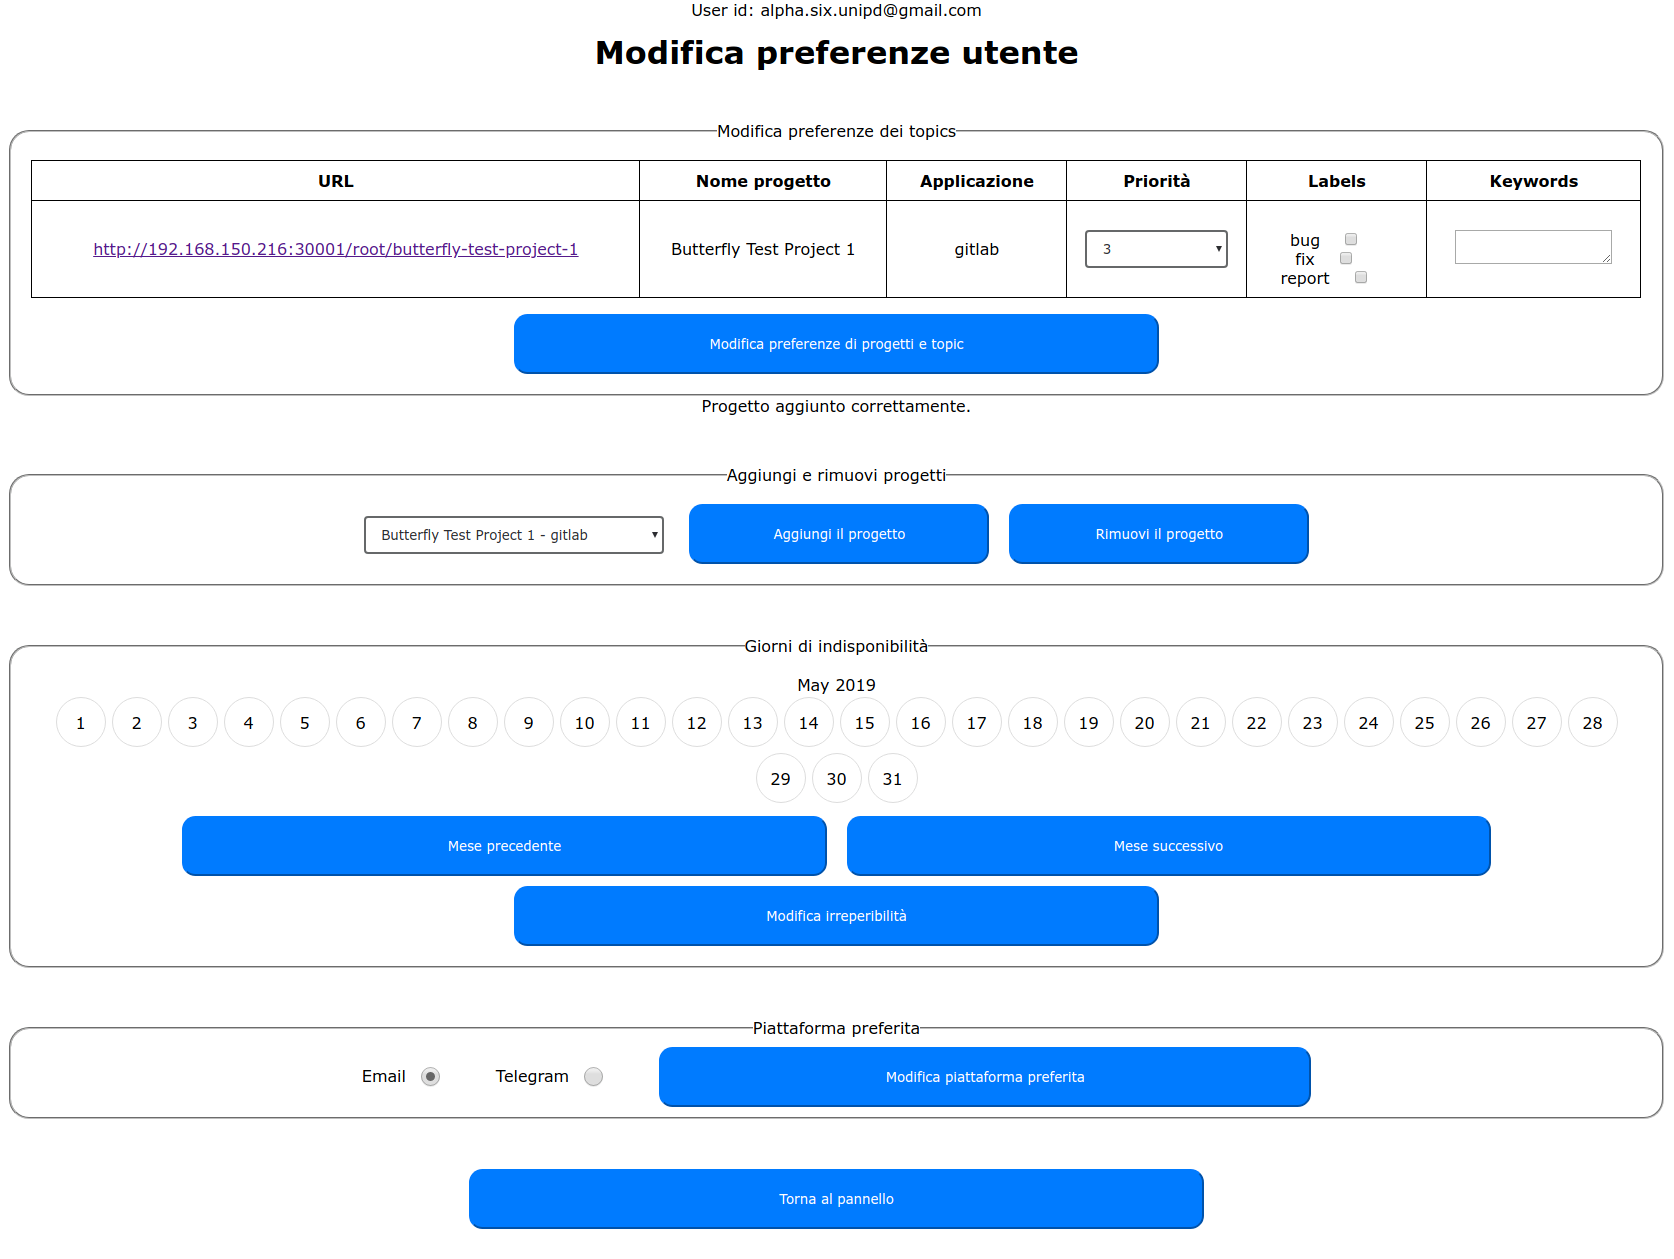
\includegraphics[width=\textwidth]{img/preferenze_1.png} %TODO verificare immagine
	\caption{Interfaccia modifica preferenze}
\end{figure}

\subsubsection{Inserimento giorni di indisponibilità}\label{indisponibilita}
Sempre dal Pannello di controllo è possibile raggiungere la pagina relativa alla disponibilità di calendario. 
%TODO verificare con Matteo
In questa è possibile specificare attraverso un calendario i giorni in cui non si è disponibili e quindi in caso di una notifica in arrivo mandarla ad un'altra persona che è in grado di gestirla.
%TODO inserire immagine di calendario
\begin{figure}[H]
	\centering
	%\includegraphics[width=\textwidth]{img/disponibilita_1.png} 
	\caption{Interfaccia iscrizione nuovo utente}
\end{figure}

\subsubsection{Uscita dal sistema}
%TODO spiegare
Per effettuare il logout dal sistema, cliccare su logout
%TODO inserire immagine

\subsubsection{Disiscrizione dal sistema}
%TODO verificare tutto
Viene data la possibilità di disiscriversi dal sistema ed eliminare quindi i propri dati all'interno di questo.
Per disiscriversi andare su ... dal pannello di controllo ...
\begin{figure}[H]
	\centering
	\includegraphics[width=10cm]{img/rimozione_1.png} %TODO verificare immagine
	\caption{Interfaccia iscrizione nuovo utente}
\end{figure}
Viene inoltre data la possibilità di disiscrivere un altro utente dal sistema facendo ...


%TODO da mettere un esempio per ciascuna
\subsection{API Rest}\label{APIRest}
\newcommand{\homeUrl}{home\_url}

Per la gestione delle risorse di \progetto\ abbiamo utilizzato lo standard architetturale delle API Rest.
Nelle sezioni successive viene descritto come interagire con le API fornite dal sistema.
Il root path sottinteso sarà sempre \texttt{\homeUrl/api/v1/}.
Ad esempio, per effettuare la GET degli user, l'indirizzo sarà:
\begin{center}
    \texttt{GET \homeUrl/api/v1/users}
\end{center}

\subsubsection{Users}

\texttt{Users} è la risorsa che corrisponde agli utenti.
È possibile visualizzare, aggiungere, modificare o rimuovere gli utenti tramite una semplice
richiesta HTTP.

\paragraph{Visualizzazione}

\begin{itemize}
    \item \textbf{Payload di tutti gli utenti}: \texttt{GET /users}
    \item \textbf{Utente specifico}: \texttt{GET /users/<id>}
\end{itemize}

\paragraph{Inserimento}
È possibile inserire un nuovo utente tramite la richiesta
    \begin{center}
        \texttt{POST /users}
    \end{center}

È possibile dare i seguenti campi di tipo stringa alla richiesta, per aggiungere in fase di creazione i dati:
\begin{itemize}[noitemsep]
    \item \texttt{name}
    \item \texttt{surname}
    \item \texttt{telegram}
    \item \texttt{email}
\end{itemize}
Almeno uno tra i campi \texttt{email} e \texttt{telegram} vanno fornite insieme al payload.

\paragraph{Modifica}

È possibile modificare un utente tramite la richiesta
\begin{center}
    \texttt{PUT /users/<id>}
\end{center}
È possibile dare i seguenti campi di tipo stringa alla richiesta, per aggiungere in fase di creazione i dati:
\begin{itemize}[noitemsep]
    \item \texttt{name}
    \item \texttt{surname}
    \item \texttt{telegram}
    \item \texttt{email}
\end{itemize}


\paragraph{Rimozione}

È possibile rimuovere un utente dal sistema \progetto\ con la richiesta
\begin{center}
    \texttt{DELETE /users/<id>}
\end{center}

Se il campo \texttt{<id>} corrisponde a un ID presente nel sistema, esso verrà rimosso.


\paragraph{Riepilogo}

\begin{table}[H]
    \begin{paddedtablex}[1.3]{\textwidth}{cYY}
        \thead{Metodo HTTP} & \thead{URI} & \thead{Action}\\\toprule
        \texttt{GET} & \texttt{/users} & Restituisce un payload in JSON di tutti gli utenti\\
        \texttt{GET} & \texttt{/users/<id>} & Restituisce un payload in JSON dell'utente che corrisponde a \texttt{<id>}\\
        \texttt{POST} & \texttt{/users} & Inserisce un nuovo utente. È necessario fornire uno tra i campi telegram o email\\
        \texttt{PUT} & \texttt{/users/<id>} & Modifica l'utente corrispondente a \texttt{<id>} con i campi passati nella richiesta\\
        \texttt{DELETE} & \texttt{/users/<id>} & Elimina l'utente corrispondente a \texttt{<id>} dal sistema\\
        \bottomrule
    \end{paddedtablex}
    \caption{Riepilogo delle Rest API per gli Users}
\end{table}


\subsubsection{Projects}

\paragraph{Visualizzazione}


\begin{itemize}
    \item \textbf{Payload di tutti i progetti}: \texttt{GET /projects}
    \item \textbf{Progetto specifico}: \texttt{GET /projects/<id>}
\end{itemize}

\paragraph{Inserimento}
È possibile inserire un nuovo progetto tramite la richiesta
    \begin{center}
        \texttt{POST /projects}
    \end{center}

È possibile dare i seguenti campi di tipo stringa alla richiesta, per aggiungere in fase di creazione
i dati:
\begin{itemize}[noitemsep]
    \item \texttt{url}
\end{itemize}


\paragraph{Modifica}

È possibile modificare un progetto tramite la richiesta
\begin{center}
    \texttt{PUT /projects/<id>}
\end{center}
È possibile dare i seguenti campi di tipo stringa alla richiesta, per aggiungere in fase di creazione
i dati:
\begin{itemize}[noitemsep]
    \item \texttt{url}
\end{itemize}


\paragraph{Rimozione}

È possibile rimuovere un progetto dal sistema Butterfly con la richiesta
\begin{center}
    \texttt{DELETE /projects/<id>}
\end{center}

Se il campo \texttt{<id>} corrisponde a un ID presente nel sistema, esso verrà rimosso.


\paragraph{Riepilogo}

\begin{table}[H]
    \begin{paddedtablex}[1.3]{\textwidth}{cYY}
        \thead{Metodo HTTP} & \thead{URI} & \thead{Action}\\\toprule
        \texttt{GET} & \texttt{/projects} & Restituisce un payload in JSON di tutti i progetti\\
        \texttt{GET} & \texttt{/projects/<id>} & Restituisce un payload in JSON del progetto che corrisponde a \texttt{<id>}\\
        \texttt{POST} & \texttt{/projects} & Inserisce un nuovo progetto\\
        \texttt{PUT} & \texttt{/projects/<id>} & Modifica il progetto corrispondente a \texttt{<id>} con i campi passati nel payload\\
        \texttt{DELETE} & \texttt{/projects/<id>} & Elimina il progetto corrispondente a \texttt{<id>} dal sistema\\
        \bottomrule
    \end{paddedtablex}
    \caption{Riepilogo delle Rest API per i progetti}
\end{table}

\subsection{Piattaforma di messaggistica}

\subsubsection{Email}

Per ricevere i messaggi di Butterfly tramite Email, è sufficiente fornire tramite l'interfaccia del Gestore Personale l'Email sulla quale si vuole ricevere la notifica.

\subsubsection{Telegram}

Per ricevere le notifiche via Telegram, è necessario fare un passaggio addizionale: va fornita l'autorizzazione al bot per poter inviare messaggi agli utenti. 
Il bot è raggiungibile al seguente link:
\begin{center}
    \url{http://t.me/ButterflyBot}
\end{center}

Dare il comando \texttt{/start} per dare l'autorizzazione di inoltro dei messaggi al bot.
È necessario inoltre aggiungere tramite l'interfaccia del Gestore Personale il proprio account Telegram.
In qualsiasi momento sarà possibile bloccare il bot in caso non si voglia più ricevere messaggi relativi a Butterfly su Telegram, tramite le funzionalità dell'applicazione.
Nel caso in cui si volesse utilizzare un altro bot, i passaggi da seguire possono essere trovati sulla pagina apposita della documentazione di Telegram\footnote{\url{https://core.telegram.org/bots}}.
%TODO aggiungere nome variabile
Per comunicare con questo bisogna modificare la variabile di ambiente ... che rappresenta il \texttt{token} univoco del nuovo bot, come descritto in \S\ref{var_consumer}.
    \section{Segnalazione problematiche}

Nel caso dovessero venire riscontrati bug o problematiche relative a \progetto, si prega di segnalarlo tramite una delle seguenti procedure:
\begin{itemize}
    \item Inviare una mail all'indirizzo \href{mailto:alpha.six.unipd@gmail.com}{alpha.six.unipd@gmail.com}. Questa deve essere nel seguente formato:
    \begin{itemize}
    	\item Oggetto: \texttt{[BUTTERFLY PROJECT]: <Nome significativo dell'evento da segnalare>}
    	\item Corpo:
    	\begin{itemize}
    		\item \texttt{[SUMMARY]: <Riepilogo di come è accaduto il fatto da segnalare>}
    		\item \texttt{[TYPE]: <Di tipo: BUG | FIX | ENHANCEMENT >}
    		\item \texttt{[PRIORITY]: <Di tipo LOW | MEDIUM | HIGH>}    		
    		\item \texttt{[SEVERITY]: <Di tipo LOW | MEDIUM | HIGH>}    		
    		\item \texttt{[DATE]: <Data in cui è stato riscontrato in formato ANNO-MESE-GIORNO>}
    		\item \texttt{[DESCRIPTION]: <Descrizione completa del fatto da segnalare>}
    		\item \texttt{[ENVIRONMENT]: <Descrizione del sistema sul quale è successo il fatto>}
   			\item \texttt{[OTHER]: <Altre informazioni utili al report e descrizione di eventuali allegati esemplificativi>}
    	\end{itemize}
    \end{itemize}
    \item Aprire una issue nel progetto \progetto\ su GitHub seguendo, come per le segnalazioni via Email, il seguente formato:
    \begin{itemize}
    	\item Titolo: \texttt{<Nome significativo dell'evento da segnalare>}
    	\item Corpo:
    	\begin{itemize}
    		\item \texttt{[SUMMARY]: <Riepilogo di come è accaduto il fatto da segnalare>}
    		\item \texttt{[TYPE]: <Di tipo: BUG | FIX | ENHANCEMENT >}
    		\item \texttt{[PRIORITY]: <Di tipo LOW | MEDIUM | HIGH>}    		
    		\item \texttt{[SEVERITY]: <Di tipo LOW | MEDIUM | HIGH>}    		
    		\item \texttt{[DATE]: <Data in cui è stato riscontrato in formato ANNO-MESE-GIORNO>}
    		\item \texttt{[DESCRIPTION]: <Descrizione completa del fatto da segnalare>}
    		\item \texttt{[ENVIRONMENT]: <Descrizione del sistema sul quale è successo il fatto>}
    		\item \texttt{[OTHER]: <Altre informazioni utili al report e descrizione di eventuali screenshot esemplificativi presenti>}
    	\end{itemize}
    \end{itemize}
    % TODO nella seconda versione da rilasciare mettere un footnote con il link al progetto in github
\end{itemize}


    \appendix
    \section{Glossario}\label{glossario}

\lettera{A}

    \parola{Adapter}{%
        Design pattern strutturale con la funzione di adattare un'interfaccia
        a un'altra, utile quando si usano oggetti di librerie esterne che
        necessitano di essere adattate alle interfacce del proprio sistema.
    }\label{Adapter}

    \parola{Applicativo}{%
        Programma software con lo scopo di rendere possibili una o più funzionalità, servizi o strumenti utili.
    }\label{Applicativo}

    \parola{API Rest}{%
        Metodi con cui è possibile fornire l'interazione con le componenti del sistema basate su representational state transfer,
        dove le risorse sono uniche e indirizzabili mediante URI.
    }\label{API Rest}

\lettera{B}

    \parola{Broker}{%
        Componente che gestisce i messaggi inviati da Publisher a Subscriber nel relativo modello architetturale.
        Mette a disposizione i \gloss{Topic} nei quali i Publisher inviano i messaggi, mentre i Subscriber possono
        iscriversi a essi per ricevere i messaggi.
    }\label{Broker}

\lettera{C}

    \parola{Cluster}{%
        È un insieme di computer connessi tra loro tramite una rete telematica. Scopo del cluster è distribuire un'elaborazione molto complessa tra i vari computer, aumentando la potenza di calcolo del sistema e/o garantendo una maggiore disponibilità di servizio, a prezzo di un maggior costo e complessità di gestione dell'infrastruttura: per essere risolto il problema che richiede molte elaborazioni viene infatti scomposto in sottoproblemi separati i quali vengono risolti ciascuno in parallelo.
    }\label{Cluster}

	\parola{Container}{% di Docker
        Consiste nella capacità di eseguire più processi e applicazioni in modo separato per sfruttare al
        meglio l'infrastruttura esistente pur conservando il livello di sicurezza che sarebbe garantito
        dalla presenza di sistemi separati.
    }\label{Container}

\lettera{D}

    \parola{Docker}{%
        Piattaforma che consente di automatizzare il \gloss{deployment} di applicazioni all'interno di \gloss{container} software.
    }\label{Docker}

    \parola{Docker-compose}{Definisce le configurazioni necessarie per come devono essere eseguite le immagini contenute nei container \gloss{Docker}, i link e le porte esposte verso l'esterno.}

    \parola{Dockerfile}{%
        Definisce le configurazioni necessarie per il container sul quale si andrà a eseguire l'\gloss{applicativo}.%
    }\label{Dockerfile}

	\parola{DockerHub}{%
        Repository di Docker che permette il versionamento delle immagini e la gestione delle build in maniera automatica innescata al push delle modifiche sulla repository del codice (necessita che queste siano collegate fra loro).
    }\label{DockerHub}

\lettera{E}

    \parola{Event Driven}{%
        È un paradigma di programmazione dell'informatica. Mentre in un programma tradizionale l'esecuzione delle istruzioni segue percorsi fissi, che si ramificano soltanto in punti ben determinati predefiniti dal programmatore, nei programmi scritti utilizzando la tecnica a eventi il flusso del programma è largamente determinato dal verificarsi di eventi esterni.
    }\label{EVM}

\lettera{F}

    \parola{Factory Method}{%
        Design Pattern creazionale, in cui l'interfaccia di creazione lascia alle sottoclassi la decisione su quale oggetto istanziare.
    }\label{Factory Method}


\lettera{J}

    \parola{JSON}{%
        Acronimo di JavaScript Object Notation, è un formato adatto all'interscambio di dati fra applicazioni client/server.
        È basato sul linguaggio JavaScript Standard ma ne è indipendente.
    }\label{JSON}

\lettera{K}

	\parola{Kubernetes}{%
        Kubernetes è uno strumento open source di orchestrazione e gestione di container. È stato sviluppato dal team di Google ed è uno dei tool più utilizzati a questo scopo. Kubernetes permette di eliminare molti dei processi manuali coinvolti nel deployment e nella scalabilità di applicazioni contenute in container e di gestire in maniera semplice ed efficiente cluster di host su cui questi vengono eseguiti.
    }\label{Kubernetes}


\lettera{M}

    \parola{Macchina virtuale}{%
        Una macchina virtuale (VM) indica un software che, attraverso un processo di virtualizzazione, crea un ambiente virtuale che emula il comportamento di una macchina fisica (PC client o server) grazie all'assegnazione di risorse hardware ed in cui alcune applicazioni possono essere eseguite come se interagissero con tale macchina.
    }\label{Macchina virtuale}

    \parola{Markdown}{%
    Linguaggio di markup con una sintassi molto semplice, convertibile in altri formati quali HTML con un \gloss{tool} omonimo.
    }\label{Markdown}

	\parola{Metadato}{%
        Particolare dato che descrive insiemi di altri dati.
    }\label{Metadato}

	\parola{MongoDB}{%
        È un \gloss{DBMS} non relazionale, orientato ai documenti. MongoDB si allontana dalla struttura tradizionale basata su tabelle dei database relazionali in favore di documenti in stile \gloss{JSON} con schema dinamico.
    }\label{MongoDB}

    \parola{MySQL}{%
        È un software di tipo server avente il compito di gestire uno o più database. Il suo compito è quello di intervenire, in qualità di intermediario, in ogni operazione sui database, gestendo gli accessi ai dati (filtrando quelli non autorizzati), ad eseguire le interrogazioni ed a restituirne il risultato ove previsto.
    }\label{MySQL}

\lettera{O}

    \parola{Open-closed principle}{%
        Principio della programmazione ad oggetti che stabilisce quanto segue: una classe dovrebbe essere aperta alle estensioni ma chiusa alle modifiche.
    }\label{Open-closed principle}

\lettera{P}

    \parola{PIP}{%
        Il Python Package Index è un repository che contiene decine di migliaia di package scritti in Python. Chiunque può scaricare package esistenti o condividere nuovi package su PIP.
    }\label{PIP}

   	\parola{Producer}{%
        Componente di Butterfly con lo scopo di raccogliere i messaggi e pubblicarli sotto forma di messaggi all'interno dei Topic adeguati.
    }\label{Producer}

\lettera{R}

	\parola{Risorsa}{%
        Soggetto consumabile che può essere di varia natura. Nel caso di un progetto software una risorsa può consistere in ore di lavoro o tecnologie utilizzabili.
    }\label{Risorsa}

\lettera{T}

    \parola{Template Method}{%
        Design pattern comportamentale che definisce la struttura di un algoritmo,
        lasciando alle sottoclassi il compito di definirne alcuni passi.
    }\label{Template Method}

    \parola{Topic}{%
        Equivalente di ``argomento'' in italiano. Nel contesto di un \gloss{Broker} si intende un canale di messaggi associato a uno specifico argomento.
    }\label{Topic}

\lettera{W}

	\parola{Webhook}{
        Metodo per aumentare o modificare il comportamento di una pagina o applicazione Web con chiamate HTTP esterne in modo semplice, standardizzato e intelligente (\gloss{callback}).
    }\label{Webhook}

    % 
\newpage
\section{Attualizzazione dei rischi} \label{AttualizzazioneDeiRischi}
    Per dar senso ai rischi posti in analisi nel \PdP forniamo un resoconto di quanti si sono effettivamente verificati nei periodi di analisi dei requisiti e di progettazione della base tecnologica.\\
    Poiché i rischi cambiano dinamicamente durante lo svolgersi del progetto, questo appendice verrà aggiornato a intervalli regolari come stabilito nelle \NdP.
    I rischi che riportiamo sono quanto effettivamente abbiamo riscontrato nel portare a compimento le attività del progetto, possono anche differire da quelli presi precedentemente in analisi.\\

	\subsection{Classificazione}
    La classificazione dei rischi avverrà in modo simile a quella usata per l'analisi, riportando in questo caso anche la data in cui è stato riscontrato il rischio.
    Viene riportata per comodità del lettore la classificazione adottata per l'analisi dei rischi.

	A ciascun rischio viene assegnato un codice identificativo in modo da essere univoco e facilmente riconoscibile.

	Questo codice è:

	\begin{center}
		\texttt{[Tipologia][ID]-[Gravità][Probabilità][Classe]-[Data]}
	\end{center}

	composto da:
	
	\begin{itemize}
		\item \textbf{Tipologia}:
			\begin{itemize}
				\item \textbf{O}: organizzativo.
				\item \textbf{P}: personale.
				\item \textbf{R}: requisiti.
				\item \textbf{S}: strumentale.
				\item \textbf{T}: tecnologico.
			\end{itemize}

		\item \textbf{ID}: numero progressivo di tre cifre che inizia da uno (001 - 999).
		\item \textbf{Gravità}:
			\begin{itemize}
				\item \textbf{0}: accettabile.
				\item \textbf{1}: tollerabile.
				\item \textbf{2}: inaccettabile.
			\end{itemize}

		\item \textbf{Probabilità}:
			\begin{itemize}
				\item \textbf{0}: bassa.
				\item \textbf{1}: media.
				\item \textbf{2}: alta.
			\end{itemize}

		\item \textbf{Classe}: ci si riferisce ai livelli di rischio individuati dalla matrice in Figura \ref{fig:rischi}
			\begin{itemize}
				\item \textbf{0}: basso (verde).
				\item \textbf{1}: medio (arancione).
				\item \textbf{2}: alto (rosso).
			\end{itemize}
			
		\item \textbf{Data}: data in cui si è verificato il rischio, nel formato riportato nelle \NdP.
	\end{itemize}

	Ad esempio, con P001-021-2018-11-10 si può capire, seguendo la legenda, che si tratta del primo rischio del personale, di gravità accettabile, probabilità alta e un valore di classe medio, verificatosi in data 2018-11-10.

	\subsection{Lista rischi riscontrati}

	Per elencare i rischi viene utilizzata una struttura tabellare che indica nella prima riga il codice identificativo e il nome di ciascun rischio,
	mentre nelle righe successive vengono elencate e discusse la relativa descrizione, le strategie per la rilevazione e le eventuali contromisure e mitigazioni.\par

	La tabella potrà essere modificata in qualsiasi momento data la dinamicità dei rischi, e si sceglie di riportarli in ordine cronologico.


	\begin{table}[H]
		\begin{risktable}{\columnwidth}{m{4cm}m{11cm}}
			\thead{P002-122-2018-11-16} &
			Impreparazione del team a livello gestionale \\
			\rowcolor{\tablegray}
			\multicolumn{2}{X}{
				\textbf{Descrizione}: ci siamo ritrovati per iniziare a svolgere le attività del progetto, partendo dallo studio di fattibilità, senza la minima conoscenza dei ruoli.
			}\\
			\multicolumn{2}{X}{
				\textbf{Strategia adottata}: ognuno ha studiato i vari ruoli e le attività da svolgere per avere una visione globale di quanto sarebbe successo.
			}\\
		\end{risktable}
		\caption{Specifica rischio P002-122-2018-11-16}
	\end{table}

	\mydoublerule{\linewidth}{0pt}{2pt}

	\begin{table}[H]
		\begin{risktable}{\columnwidth}{m{4cm}m{11cm}}
			\thead{P003-122-2019-01-13} &
			Verifica e approvazione errata di documenti \\
			\rowcolor{\tablegray}
			\multicolumn{2}{X}{
				\textbf{Descrizione}: si sono verificate delle sviste durante la verifica dei documenti e l'approvazione è stata di conseguenza errata.
			}\\
			\multicolumn{2}{X}{
				\textbf{Strategia adottata}: abbiamo ricontrollato i documenti con più attenzione. Servirà dedicare più tempo alle attività di verifica.
			}\\
		\end{risktable}
		\caption{Specifica rischio P003-122-2019-01-13}
	\end{table}

	\mydoublerule{\linewidth}{0pt}{2pt}
	
	\begin{table}[H]
		\begin{risktable}{\columnwidth}{m{4cm}m{11cm}}
			\thead{S001-100-2019-01-18} &
			Problematiche hardware \\

			\rowcolor{\tablegray}
			\multicolumn{2}{X}{
				\textbf{Descrizione}: lo schermo del pc destinato alla presentazione è rimasto privo della retroilluminazione.
			}\\

			\multicolumn{2}{X}{
				\textbf{Strategia adottata}: abbiamo usato il pc di un altro membro del gruppo.
			}\\
		\end{risktable}
		\caption{Specifica rischio S001-100-2019-01-18}		
	\end{table}

	\mydoublerule{\linewidth}{0pt}{2pt}
	
	\begin{table}[H]
		\begin{risktable}{\columnwidth}{m{4cm}m{11cm}}
			\thead{O002-111-2019-02-09} &
			Mancanza di comunicazione con l'azienda \\

			\rowcolor{\tablegray}
			\multicolumn{2}{X}{
				\textbf{Descrizione}: la mancanza di una comunicazione abbastanza approfondita con la proponente ci ha portato a dover rivedere nel dettaglio i casi d'uso dell'\AdR.
			}\\

			\multicolumn{2}{X}{
				\textbf{Strategia adottata}: abbiamo previsto più momenti in cui comunicare con l'azienda, in modo da evitare ulteriori malintesi.
			}\\
		\end{risktable}
		\caption{Specifica rischio O002-111-2019-02-09}	
	\end{table}

	\mydoublerule{\linewidth}{0pt}{2pt}

	\begin{table}[H]

		\begin{risktable}{\columnwidth}{m{4cm}m{11cm}}
			\thead{P007-122-2019-02-12} &
			Pianificazione errata dei tempi \\
			\rowcolor{\tablegray}
			\multicolumn{2}{X}{
				\textbf{Descrizione}: ci siamo ritrovati con alcuni membri che avevano tutti gli esami previsti per il terzo anno da ultimare, altri con influenza e febbre. Questo ha portato a un ritardo non previsto nello svolgimento delle attività.
			}\\

			\multicolumn{2}{X}{
				\textbf{Strategia adottata}: abbiamo usato gli strumenti di pianificazione e coordinazione quali GitHub e Slack per coordinarci meglio e gestire il lavoro da ultimare.
			}\\
		\end{risktable}
		\caption{Specifica rischio P007-122-2019-02-12}
	\end{table}
    
	
	In seguito poniamo i rischi analizzati la cui priorità è cambiata nel corso del progetto:
	\begin{itemize}
	    \item \textbf{P005-011}: Intesa parziale tra i membri del team di sviluppo.
	    \item \textbf{R001-111}: Interpretazione errata dei requisiti: aggiunta o modifica di requisiti in corso di sviluppo.
	\end{itemize}

\end{document}
